\documentclass[aspectratio=169,10pt]{beamer}
\usetheme{Boadilla}
\usepackage{graphicx,booktabs,array}
\newcommand{\Lg}{\Lambda_b\!\to\!\Lambda\gamma}
\newcommand{\ct}{\cos\theta_p}
\newcommand{\fig}[2]{\begin{frame}{#1}\centering\includegraphics[width=.98\textwidth,height=.79\textheight,keepaspectratio]{figures/#2}\end{frame}}
\title{Reconstructing $\Lg$ at FCC-ee}
\subtitle{Stage 1 v3, XGBoost and three-flavour peak optimization}
\author{FCC-ee $\Lambda_b\to\Lambda\gamma$ analysis}
\date{4 October 2026}
\begin{document}
\frame{\titlepage}

\begin{frame}{Physics goal and analysis chain}
\begin{itemize}
\item Reconstruct $\Lambda_b\to\Lambda(p\pi)\gamma$ and eventually fit the selected $\ct$ distribution with a generated-to-reconstructed efficiency and response.
\item Chain: named EvtGen decay $\to$ Delphes IDEA response $\to$ Stage 1 candidate building $\to$ Stage 2 offline preselection $\to$ Zbb-trained XGBoost $\to$ reconstructed misidentification and photon-pair checks.
\item Project the 5.4--5.9 GeV reconstructed signal peak at $6\times10^{12}$ Z decays. Keep signal, wrong combinations, inclusive flavours and forced physics modes distinct.
\item All charge conjugates are included. MC identity is attached \emph{after} candidate construction, and is used for diagnostics and signal counting only.
\end{itemize}
\end{frame}

\begin{frame}{Frozen v3 samples and denominators}
\small\begin{tabular}{lrrl}
\toprule
Sample & Input events & Generated direct decays & Role\\\midrule
Physics $\Lg$ & 100,000 & 100,002 & training signal / yield\\
PHSP $\Lg$ & 100,000 & 100,007 & angular acceptance\\
Inclusive Zbb & 395,623,929 & --- & 1,091 validated chunks\\
Inclusive Zcc & 499,786,495 & --- & 1,200 validated chunks\\
Inclusive Zss & 499,842,440 & --- & 1,200 validated chunks\\
Forced $\Lambda\eta$ & 100,000 & 100,000 & dedicated physics response\\
Forced $\Lambda\pi^0$ & 100,000 & 100,005 & dedicated physics response\\
\bottomrule\end{tabular}
\vspace{.5em}

\scriptsize v3 denotes the reconstruction scenario, not the Stage 0 EDM4hep generator label. Candidate rows and candidate-bearing events have separate counters. Forced modes cannot be added blindly to inclusive Zbb.
\end{frame}

\begin{frame}{Stage 1: candidate construction from reconstructed objects}
\begin{enumerate}
\item Choose the primary vertex and reconstructed photon; form opposite-charge track pairs, fit a displaced $\Lambda$ vertex and test both $p\pi$ mass assignments.
\item Retain a good SV ($\chi^2\leq9$), daughter $|d_0|/\sigma\geq3$, PV--SV flight $\geq0.3$ mm and significance $\geq2$, $|m(p\pi)-m_\Lambda|\leq15$ MeV.
\item Combine the $\Lambda$ and photon in the same thrust hemisphere, $4.5\leq m(\Lambda\gamma)\leq6.5$ GeV; write all candidate observables and keys.
\item Stage 2 keeps $|m(p\pi)-m_\Lambda|\leq12.5$ MeV, $E_{\Lambda_b}\geq10.5$ GeV and $4.7\leq m(\Lambda\gamma)\leq6.5$ GeV. No photon veto enters this offline baseline.
\end{enumerate}
\scriptsize One candidate per downstream row: event entry, candidate slot and candidates in event. Unselected rows are kept for cut studies.
\end{frame}

\begin{frame}{What is measured around one candidate?}
\centering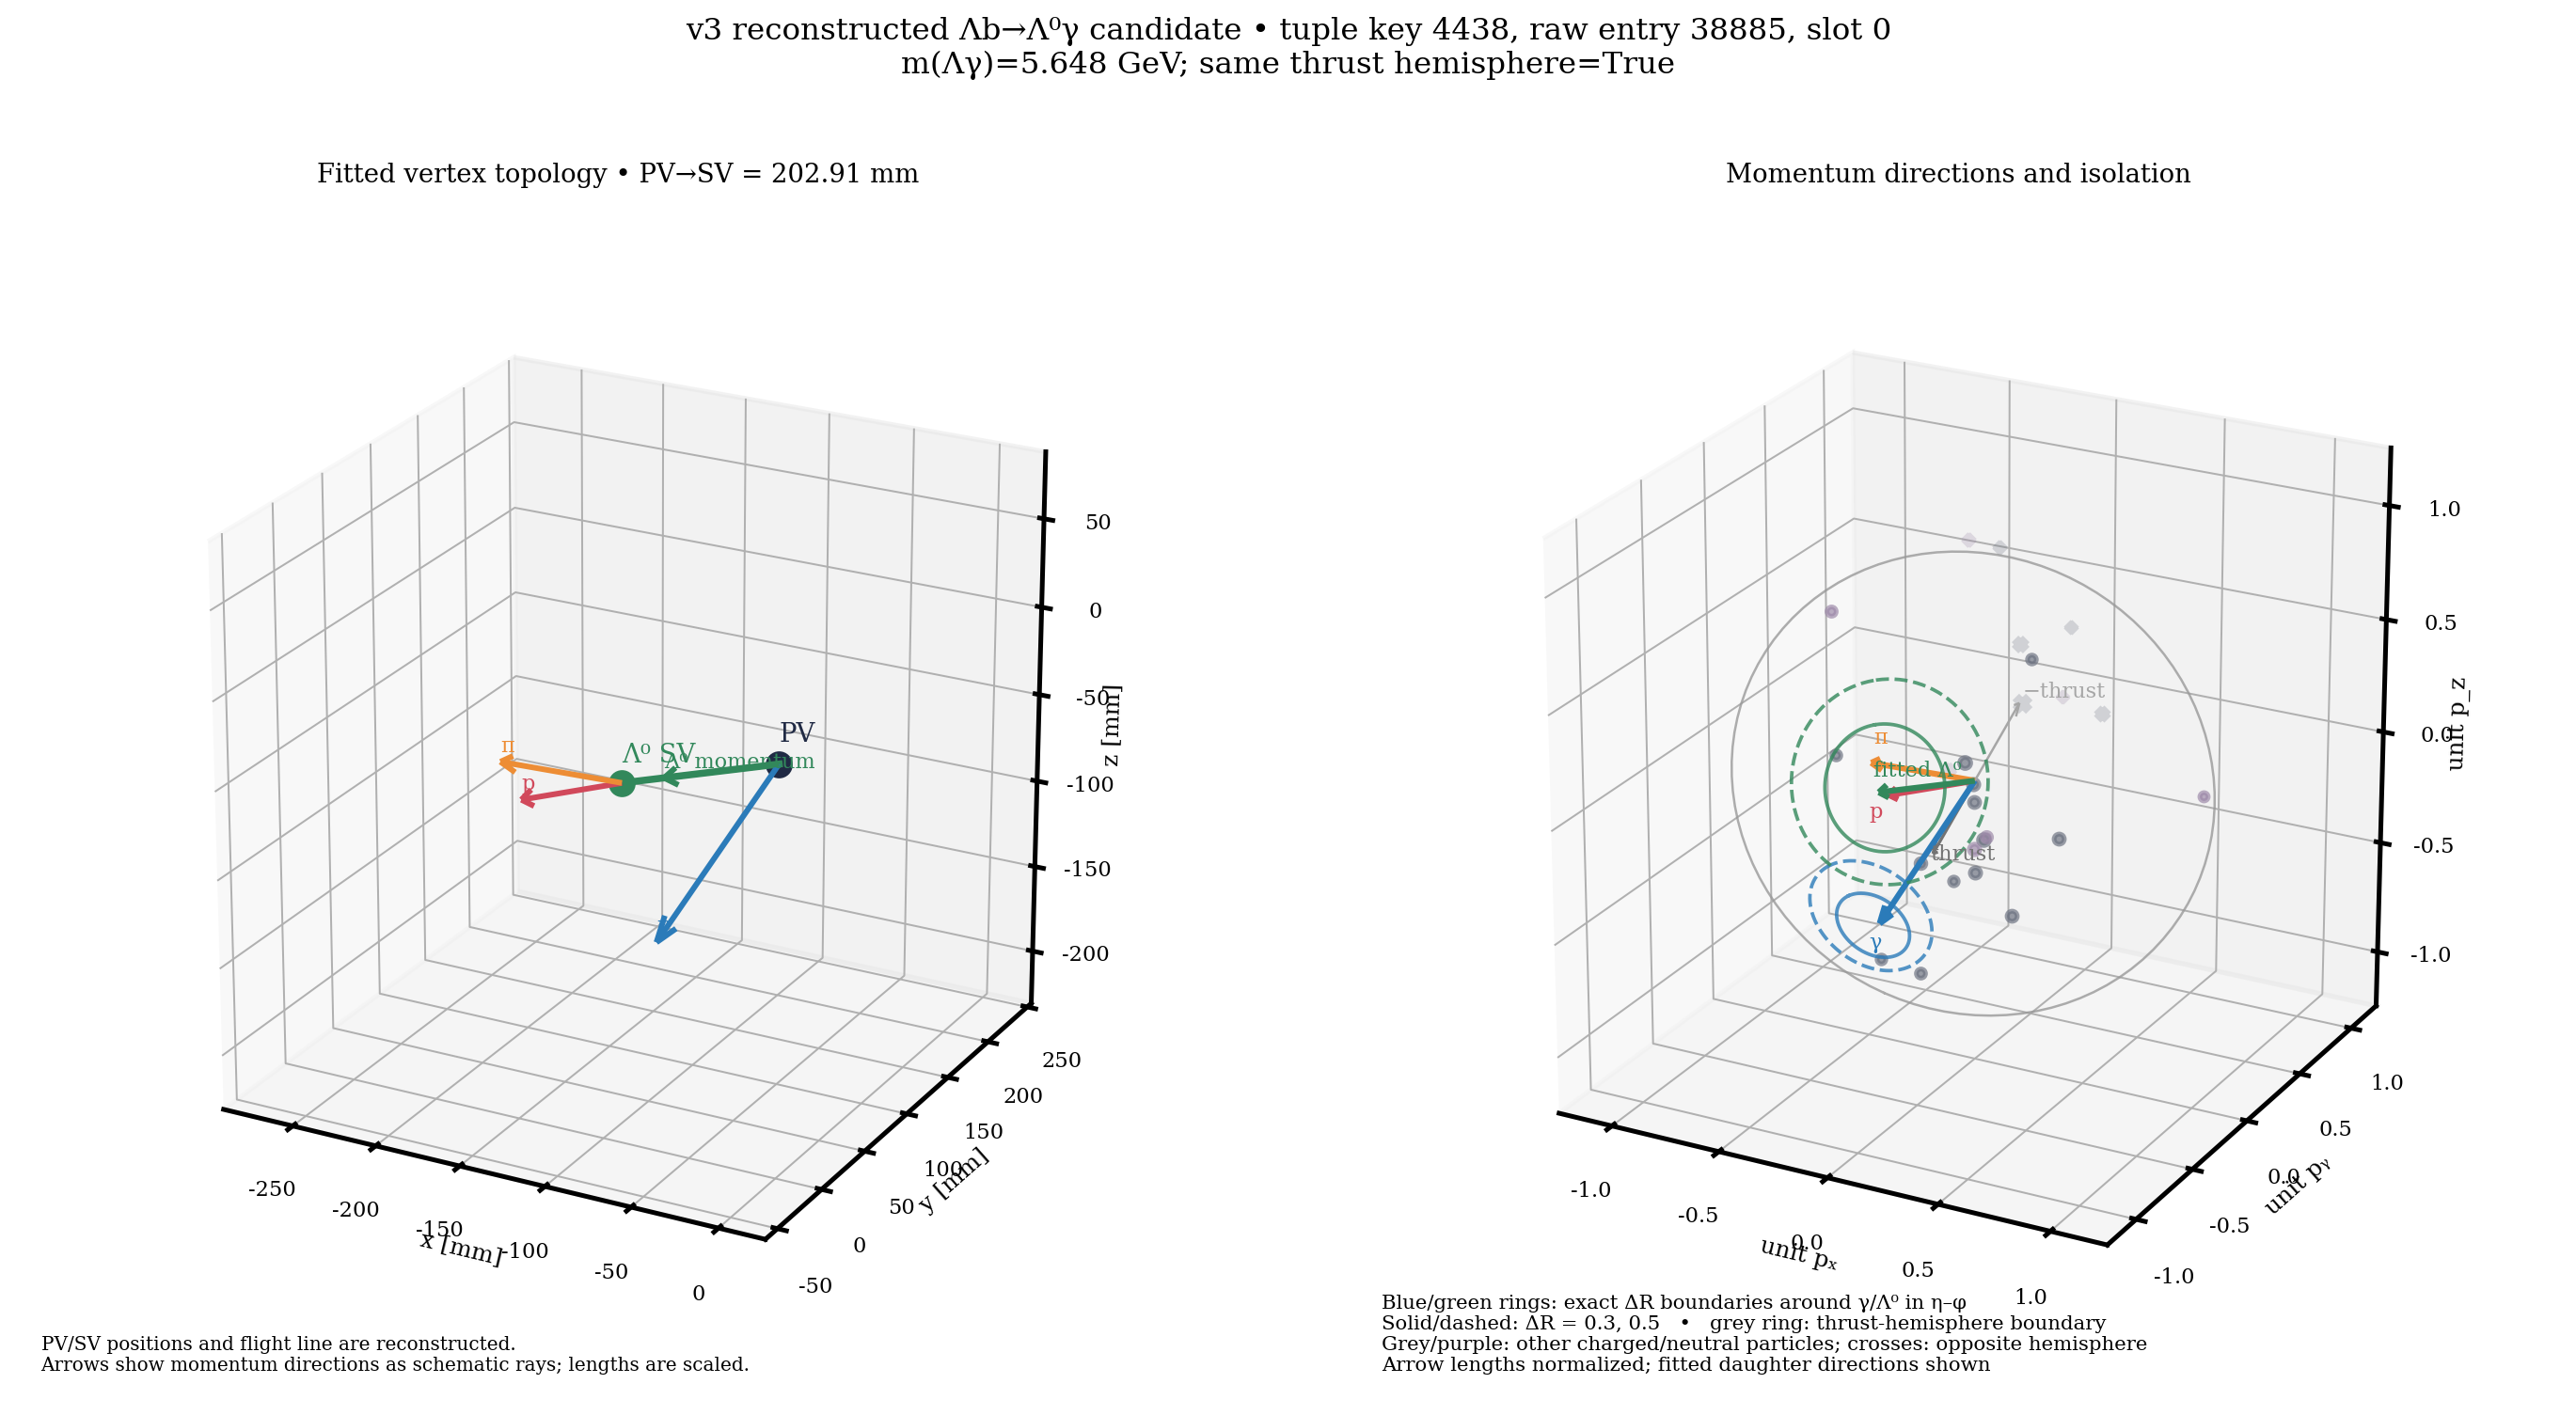
\includegraphics[width=.92\textwidth,height=.72\textheight,keepaspectratio]{figures/candidate_3d_view_a.png}
\scriptsize Schematic event display: PV, displaced $\Lambda$ SV, proton/pion trajectories, candidate photon and isolation cones. Geometry illustrates definitions; it is not a detector event.
\end{frame}

\begin{frame}{Stage 1 observable families and construction}
\small\begin{tabular}{p{.25\textwidth}p{.67\textwidth}}
\toprule
Family & Reconstructed definition / physical role\\\midrule
Kinematics & $p_p,p_\pi,p_\Lambda,E_\gamma,E_{\Lambda_b}$; partial recoil energy/momentum imbalance relative to event hemispheres.\\
Vertex and topology & Daughter $d_0/\sigma$, PV--SV 3D flight significance; thrust-axis alignment of $\Lambda_b$.\\
Isolation and activity & Energy/counts in $\Delta R=0.2,0.3,0.5,0.7,1,2$ around photon/$\Lambda$; exclude candidate daughters; include displaced neighbour-track counts.\\
Photon partner & Pair candidate photon with raw same-hemisphere photon; store closest $\pi^0$ and $\eta$ mass distances and minimum $m_{\gamma\gamma}$. Empty partner lists are retained.\\
Pair identity & Armenteros $\alpha=(p_L^+-p_L^-)/(p_L^++p_L^-)$ and $q_T$; computed from reconstructed daughter momenta.\\
\bottomrule\end{tabular}
\vspace{.3em}

\scriptsize MC parent, grandparent and earlier ancestor fields are appended after reconstruction; none defines candidate or BDT inputs.
\end{frame}

\fig{Before BDT: kinematic variables in the peak (unit shapes)}{pre_bdt_peak_kinematics.png}
\fig{Before BDT: isolation and activity in the peak (unit shapes)}{pre_bdt_peak_activity.png}
\fig{Before BDT: displaced topology in the peak (unit shapes)}{pre_bdt_peak_topology.png}

\begin{frame}{Frozen XGBoost: 20 reconstructed inputs}
\scriptsize\begin{tabular}{p{.46\textwidth}p{.46\textwidth}}
\toprule
Kinematics and vertex & Isolation, event shape and photon partners\\\midrule
$E_{\Lambda_b},p_p,p_\pi,E_\gamma,p_\Lambda$ & $|\cos\theta(\Lambda_b,\mathrm{thrust})|$\\
$d_0(p)/\sigma, d_0(\pi)/\sigma$ & $E_{\rm all}^{R<.3}(\gamma)/E_\gamma$\\
PV--SV flight significance & $N_{\rm charged}^{R<.5}(\gamma)$\\
Partial $\Delta E$, partial $\Delta p$ & $N_{\rm neutral}^{R<.3}(\gamma)$\\
 & $N_{\rm charged}^{R<.5}(\Lambda; d_0)$\\
 & min/max $|d_0|$ of $\Lambda$ neighbours\\
 & $|m_{\gamma\gamma}-m_{\pi^0}|$, $|m_{\gamma\gamma}-m_\eta|$, min $m_{\gamma\gamma}$\\
\bottomrule\end{tabular}
\vspace{1em}

\small Config: \texttt{v3\_offline\_no\_veto\_proposal}. Isolation removes candidate daughters. Photon-partner distances have a no-partner sentinel. Mass $m(\Lambda\gamma)$, $\ct$, truth and candidate keys are excluded from training.
\end{frame}

\begin{frame}{Training and held-out checks}
\begin{itemize}
\item Train direct Physics truth-matched candidates versus nonmatched inclusive Zbb candidates after the same Stage 2 offline selection. Entire Zbb chunks and signal event hashes stay within one partition.
\item The frozen model used 1,091 Zbb chunks, 8 parallel Parquet readers and 16 XGBoost threads. ROC AUC: train 0.998735, validation 0.998617, test 0.998519.
\item Model score, feature order, plots, preparation catalog and uncut scored shards are frozen. The 0.953827 score came from the earlier Zbb-only peak scan.
\item Current question: can a different threshold improve the \emph{same model} once Zcc and Zss are projected too? A new weighted-mixture model is a separate next study.
\end{itemize}
\end{frame}

\begin{frame}{Frozen model checks}
\centering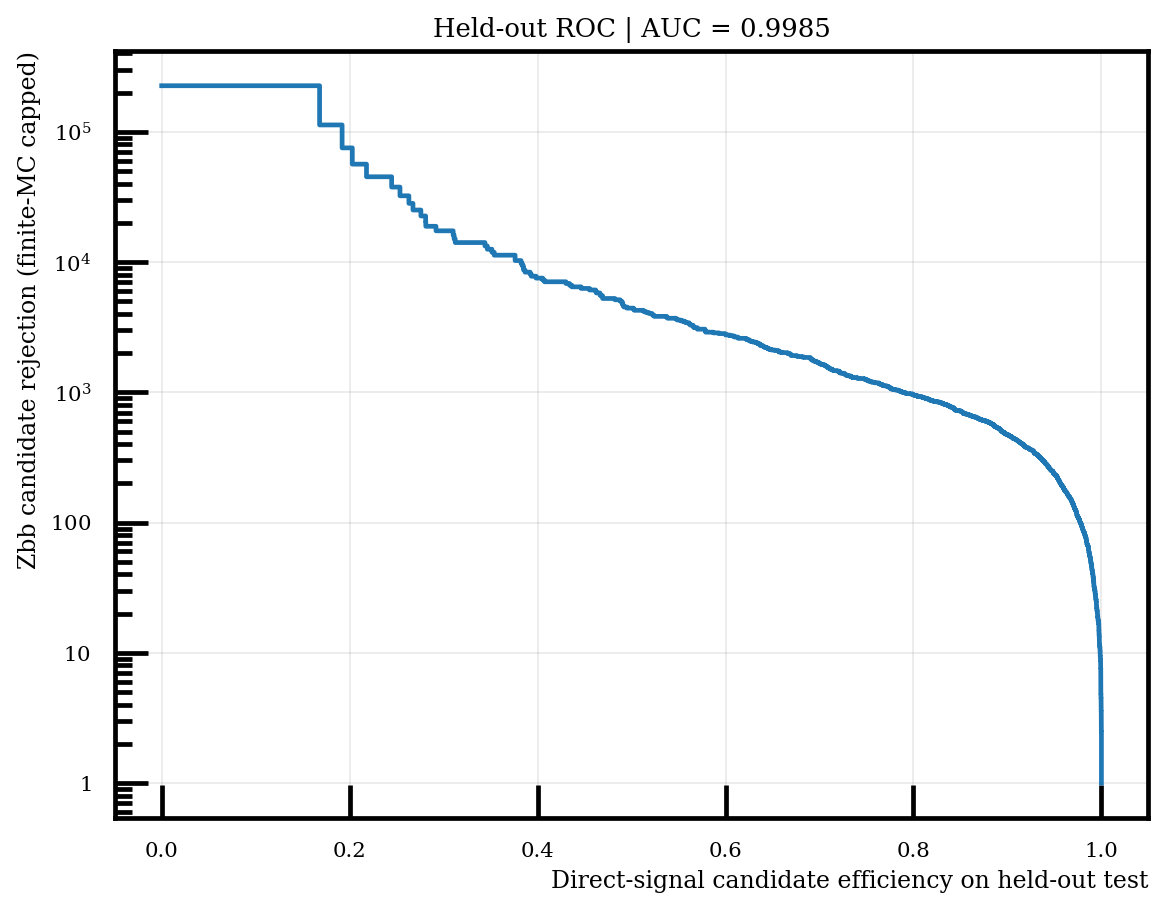
\includegraphics[width=.49\textwidth,height=.72\textheight,keepaspectratio]{figures/test_roc.png}\hfill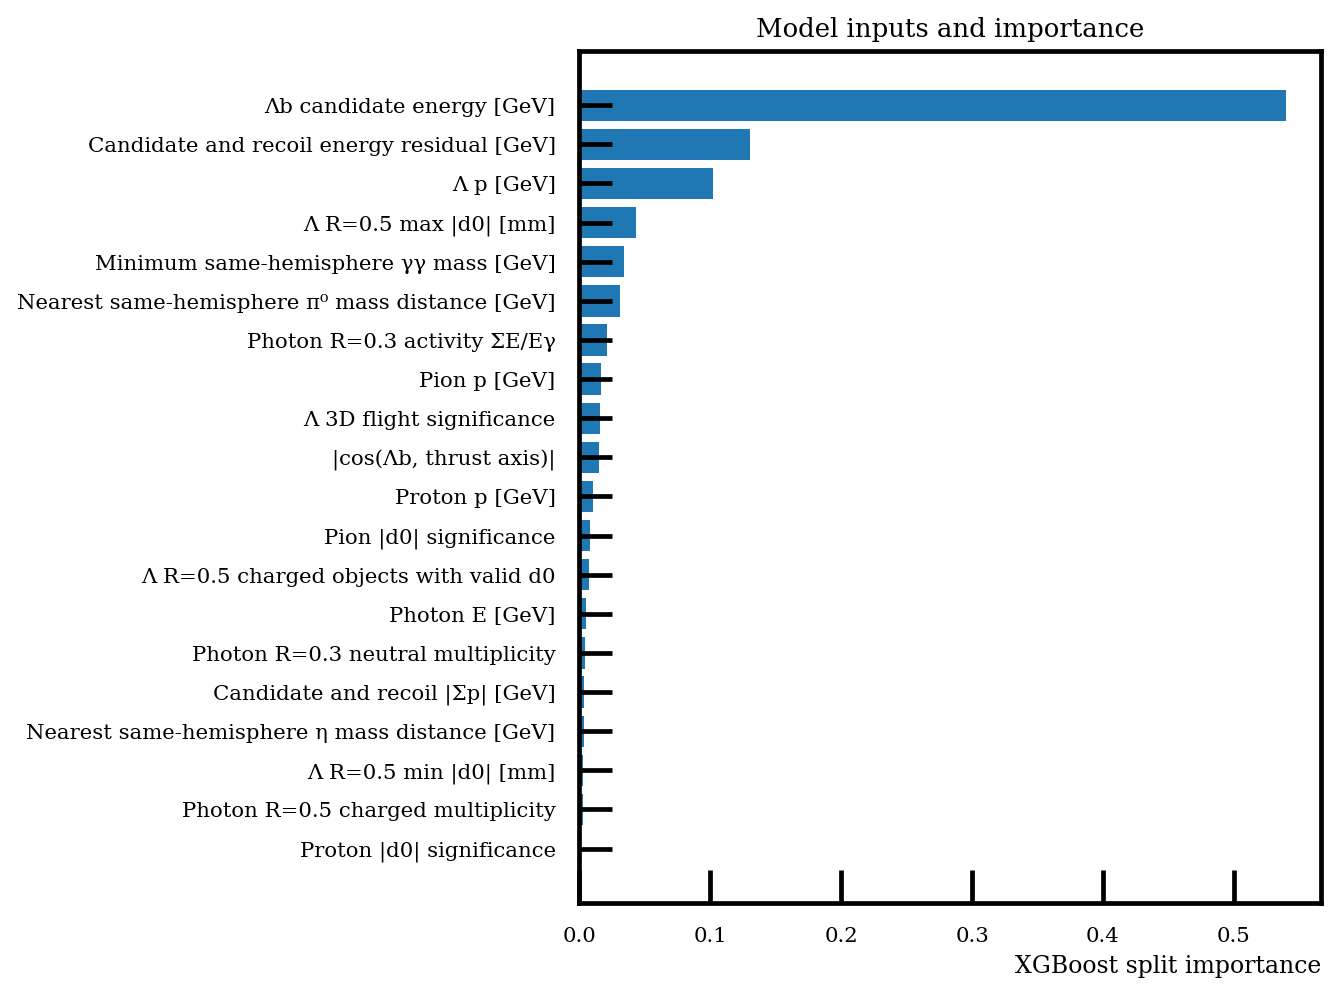
\includegraphics[width=.49\textwidth,height=.72\textheight,keepaspectratio]{figures/feature_importance.png}
\scriptsize Left: held-out Zbb-only classification ROC. Right: frozen model feature importance; these are model diagnostics, not a three-flavour performance estimate.
\end{frame}

\begin{frame}{Armenteros: testing $K_S^0\to\pi\pi$ misidentification}
\centering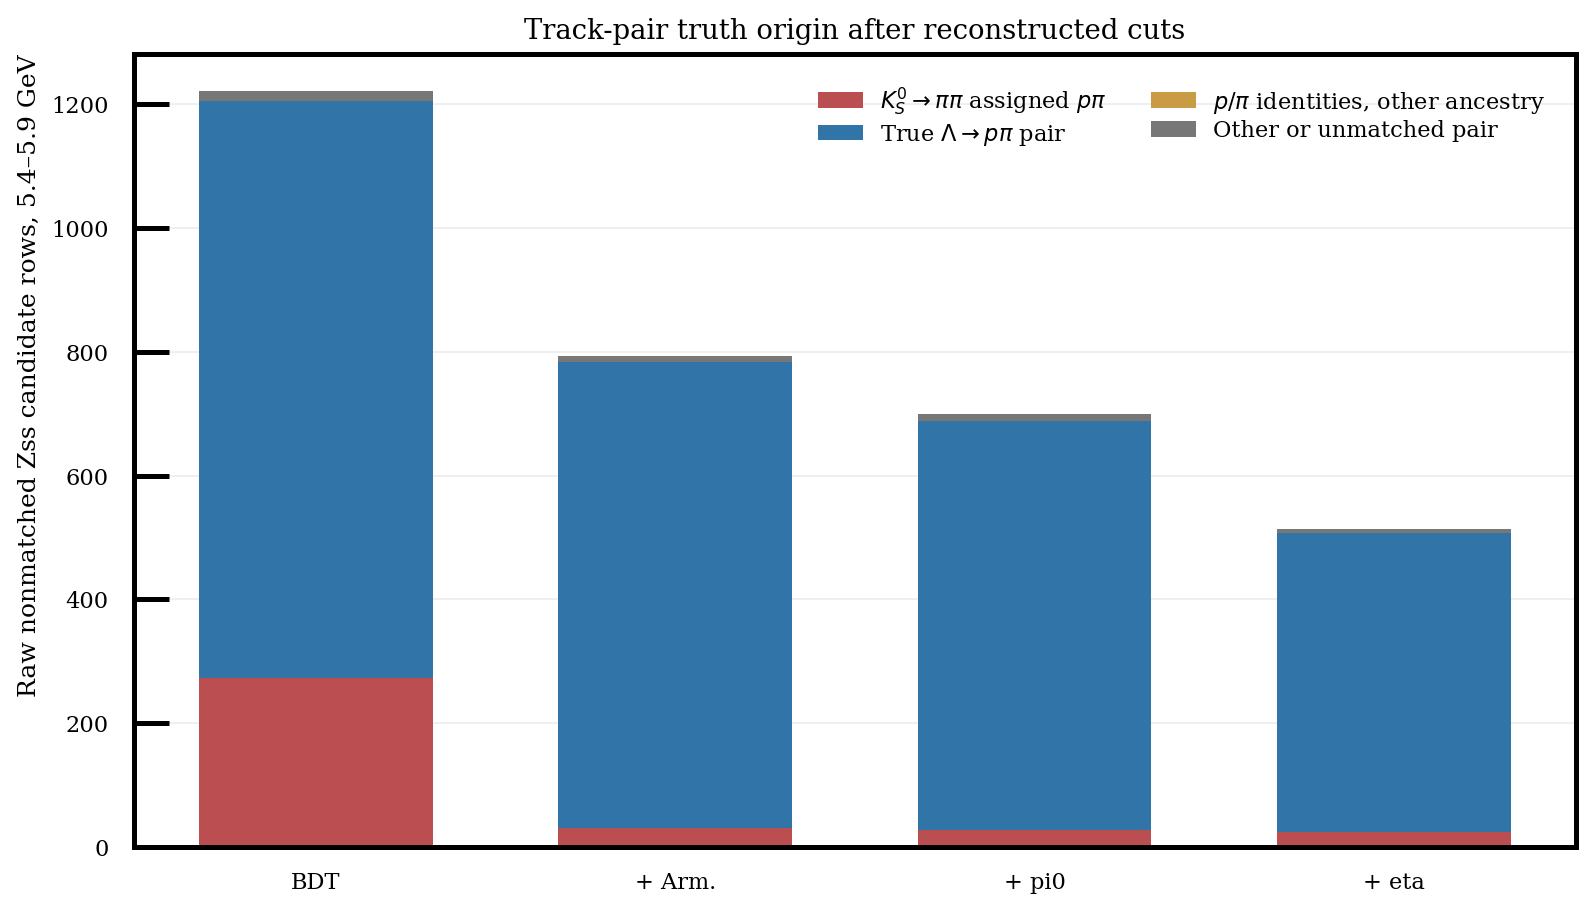
\includegraphics[width=.75\textwidth,height=.63\textheight,keepaspectratio]{figures/zss_peak_pair_origin.png}
\scriptsize Fixed BDT 0.953827, Zss peak: 273 true $K_S^0$ pairs $\to$31 after rejecting $0.67\leq|\alpha|\leq0.78$, $0.075\leq q_T\leq0.120$ GeV (88.6\% removed). True $\Lambda$ pairs: 932 $\to$752. Signal peak: 36,900 $\to$28,345 raw direct candidates. Truth categories diagnose the reconstructed cut.
\end{frame}

\begin{frame}{Photon-pair veto mechanics and observed effects}
\small\begin{itemize}
\item Search additional raw type-22 photons on the candidate $\Lambda$ thrust hemisphere. Reject if the nearest reconstructed $m(\gamma\gamma)$ lies within 20 MeV of $m_{\pi^0}$ or 50 MeV of $m_\eta$. No eligible partner means no veto.
\item At old BDT+Armenteros, sequential $\pi^0$ veto: expected signal 231,473$\to$228,827 and Zss 1,486,837$\to$1,308,940 in the peak. Then $\eta$ veto: signal $\to$194,757; Zss $\to$962,511.
\item Forced $\Lambda\eta$ estimate: 9,844$\to$9,785$\to$1,924; forced $\Lambda\pi^0$: 84$\to$66$\to$60. These are separately normalized sensitivity projections.
\end{itemize}
\scriptsize These windows are named proposals, not part of Stage 1 or the BDT score. The $\eta$ step removes sizeable direct signal.
\end{frame}

\begin{frame}{Forced $\Lambda\pi^0$ and $\Lambda\eta$ response (100k each)}
\centering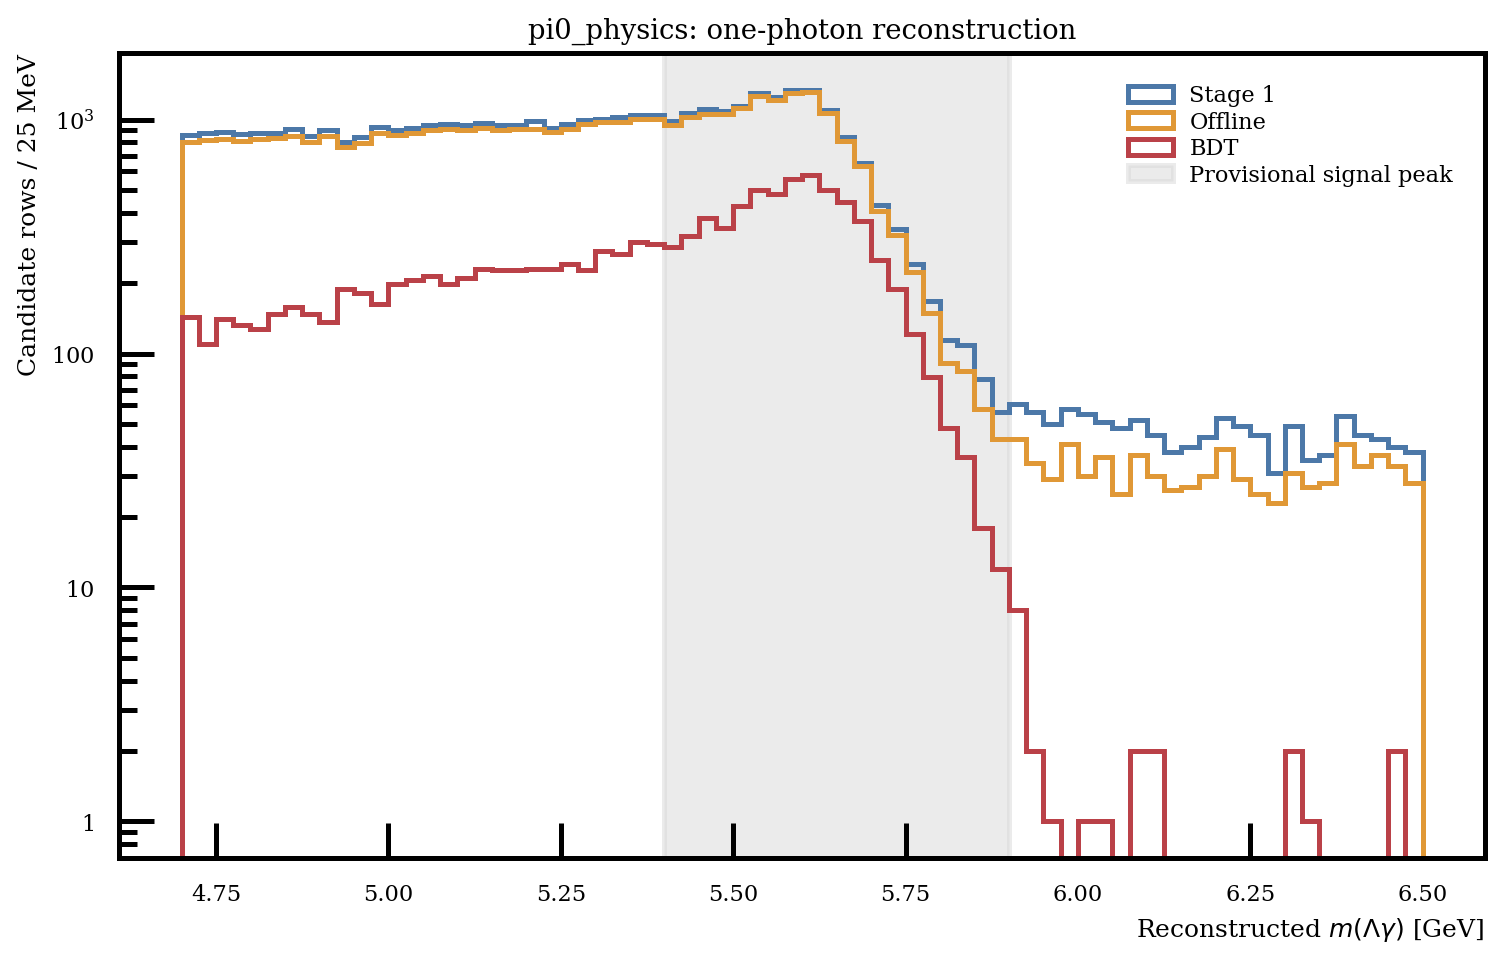
\includegraphics[width=.49\textwidth,height=.70\textheight,keepaspectratio]{figures/pi0_physics_mass_cutflow.png}\hfill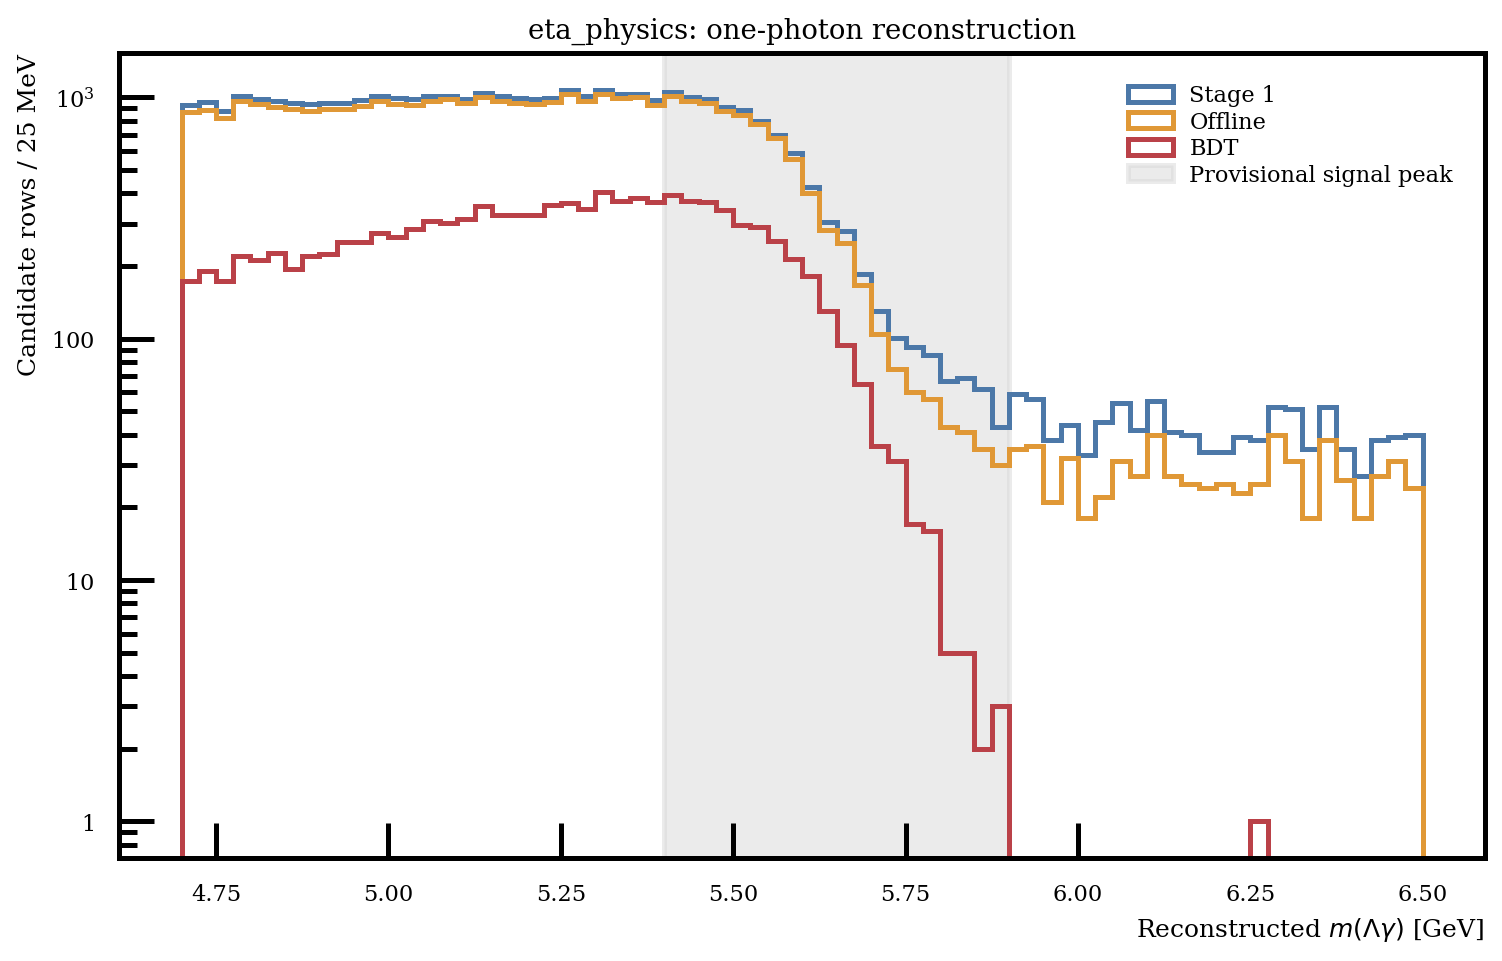
\includegraphics[width=.49\textwidth,height=.70\textheight,keepaspectratio]{figures/eta_physics_mass_cutflow.png}
\scriptsize Reconstructed candidate mass cutflows, one-photon Stage 1 v3 scenario. Forced samples test veto response; their projected yields are not additional inclusive Zbb components.
\end{frame}

\begin{frame}{Why Zcc and Zss matter}
\small\begin{tabular}{lrrr}
\toprule
Old 0.953827 score, peak & Zbb & Zcc & Zss\\\midrule
Raw rows after BDT & --- & 469 & 1,221\\
Expected after BDT & 550,523 & 677,338 & 2,286,433\\
Expected after Armenteros & 79,621 & 410,158 & 1,486,837\\
Expected after both photon vetoes & 61,422 & 363,943 & 962,511\\
\bottomrule\end{tabular}
\vspace{.8em}

\begin{itemize}
\item Scale each flavour with its own processed-event denominator and $\mathcal B(Z\to q\bar q)$. For Zss, 0.156 is an explicit equal-down-type scenario.
\item After all vetoes, 483/514 Zss peak rows still have a genuine $\Lambda$ pair; 352/514 selected photons have an immediate recorded $s$-quark parent. Armenteros cannot remove this genuine-$\Lambda$ component.
\end{itemize}
\end{frame}

\begin{frame}{First score scan: the unchanged BDT and three backgrounds}
\small\begin{enumerate}
\item Keep the Zbb-trained model and score for each scored row. Apply reconstructed Armenteros alone, Armenteros+$\eta$, and $\pi^0$ controls on the same rows.
\item In the 5.4--5.9 GeV peak, scale direct signal by generated direct decays; scale Zbb, Zcc and Zss separately by $N_Z\mathcal B_q/N_{\rm processed,q}$.
\item First scan every observed validation score for $S/\sqrt{S+B_{bb}+B_{cc}+B_{ss}}$, then evaluate that fixed score on held-out test partitions. The PI subsequently requested a separate $S/\sqrt{B}$ scan at tighter scores. No MC ancestry is an input cut.
\end{enumerate}
\scriptsize $N_Z=6\times10^{12}$, $\mathcal B_{bb}=0.15$, $\mathcal B_{cc}=0.1203$, $\mathcal B_{ss}=0.156$. Forced modes and wrong signal combinations are shown separately, not included in this exact objective.
\end{frame}

\fig{Earlier objective: three-flavour $S/\sqrt{S+B}$ versus score}{three_flavour_fom_score_scan.png}

\begin{frame}{Earlier $S/\sqrt{S+B}$ validation choice and held-out test}
\small\begin{tabular}{lrrrr}
\toprule
Selection & Score & Validation FoM & Test FoM & Test $S/(S+B)$\\\midrule
Armenteros, old & .953827 & 147.8 & 157.5 & 10.8\%\\
Armenteros, proposed & \textbf{.985562} & \textbf{189.3} & \textbf{174.5} & 20.5\%\\
Armenteros+$\eta$, old & .953827 & 136.9 & 153.1 & 12.0\%\\
Armenteros+$\eta$, proposed & .984990 & 178.0 & 167.5 & 21.0\%\\
Armenteros+$\pi^0$, exploratory & .984588 & 193.2 & 182.4 & 21.8\%\\
\bottomrule\end{tabular}
\vspace{.8em}

\small Armenteros-only test FoM improves 10.9\% over the old threshold. The $\eta$ veto lowers the optimized FoM. The $\pi^0$ control is promising but needs acceptance and forced-mode review.

\scriptsize At the Armenteros-only validation optimum there are only 1 Zbb, 5 Zcc, 21 Zss peak rows. Counting, branching and detector uncertainties constrain any claim of an optimum.
\end{frame}

\fig{Peak signal and each inclusive flavour versus score}{three_flavour_peak_yields_score_scan.png}

\begin{frame}{Earlier 0.985562 score: candidate fit view + Armenteros}
\centering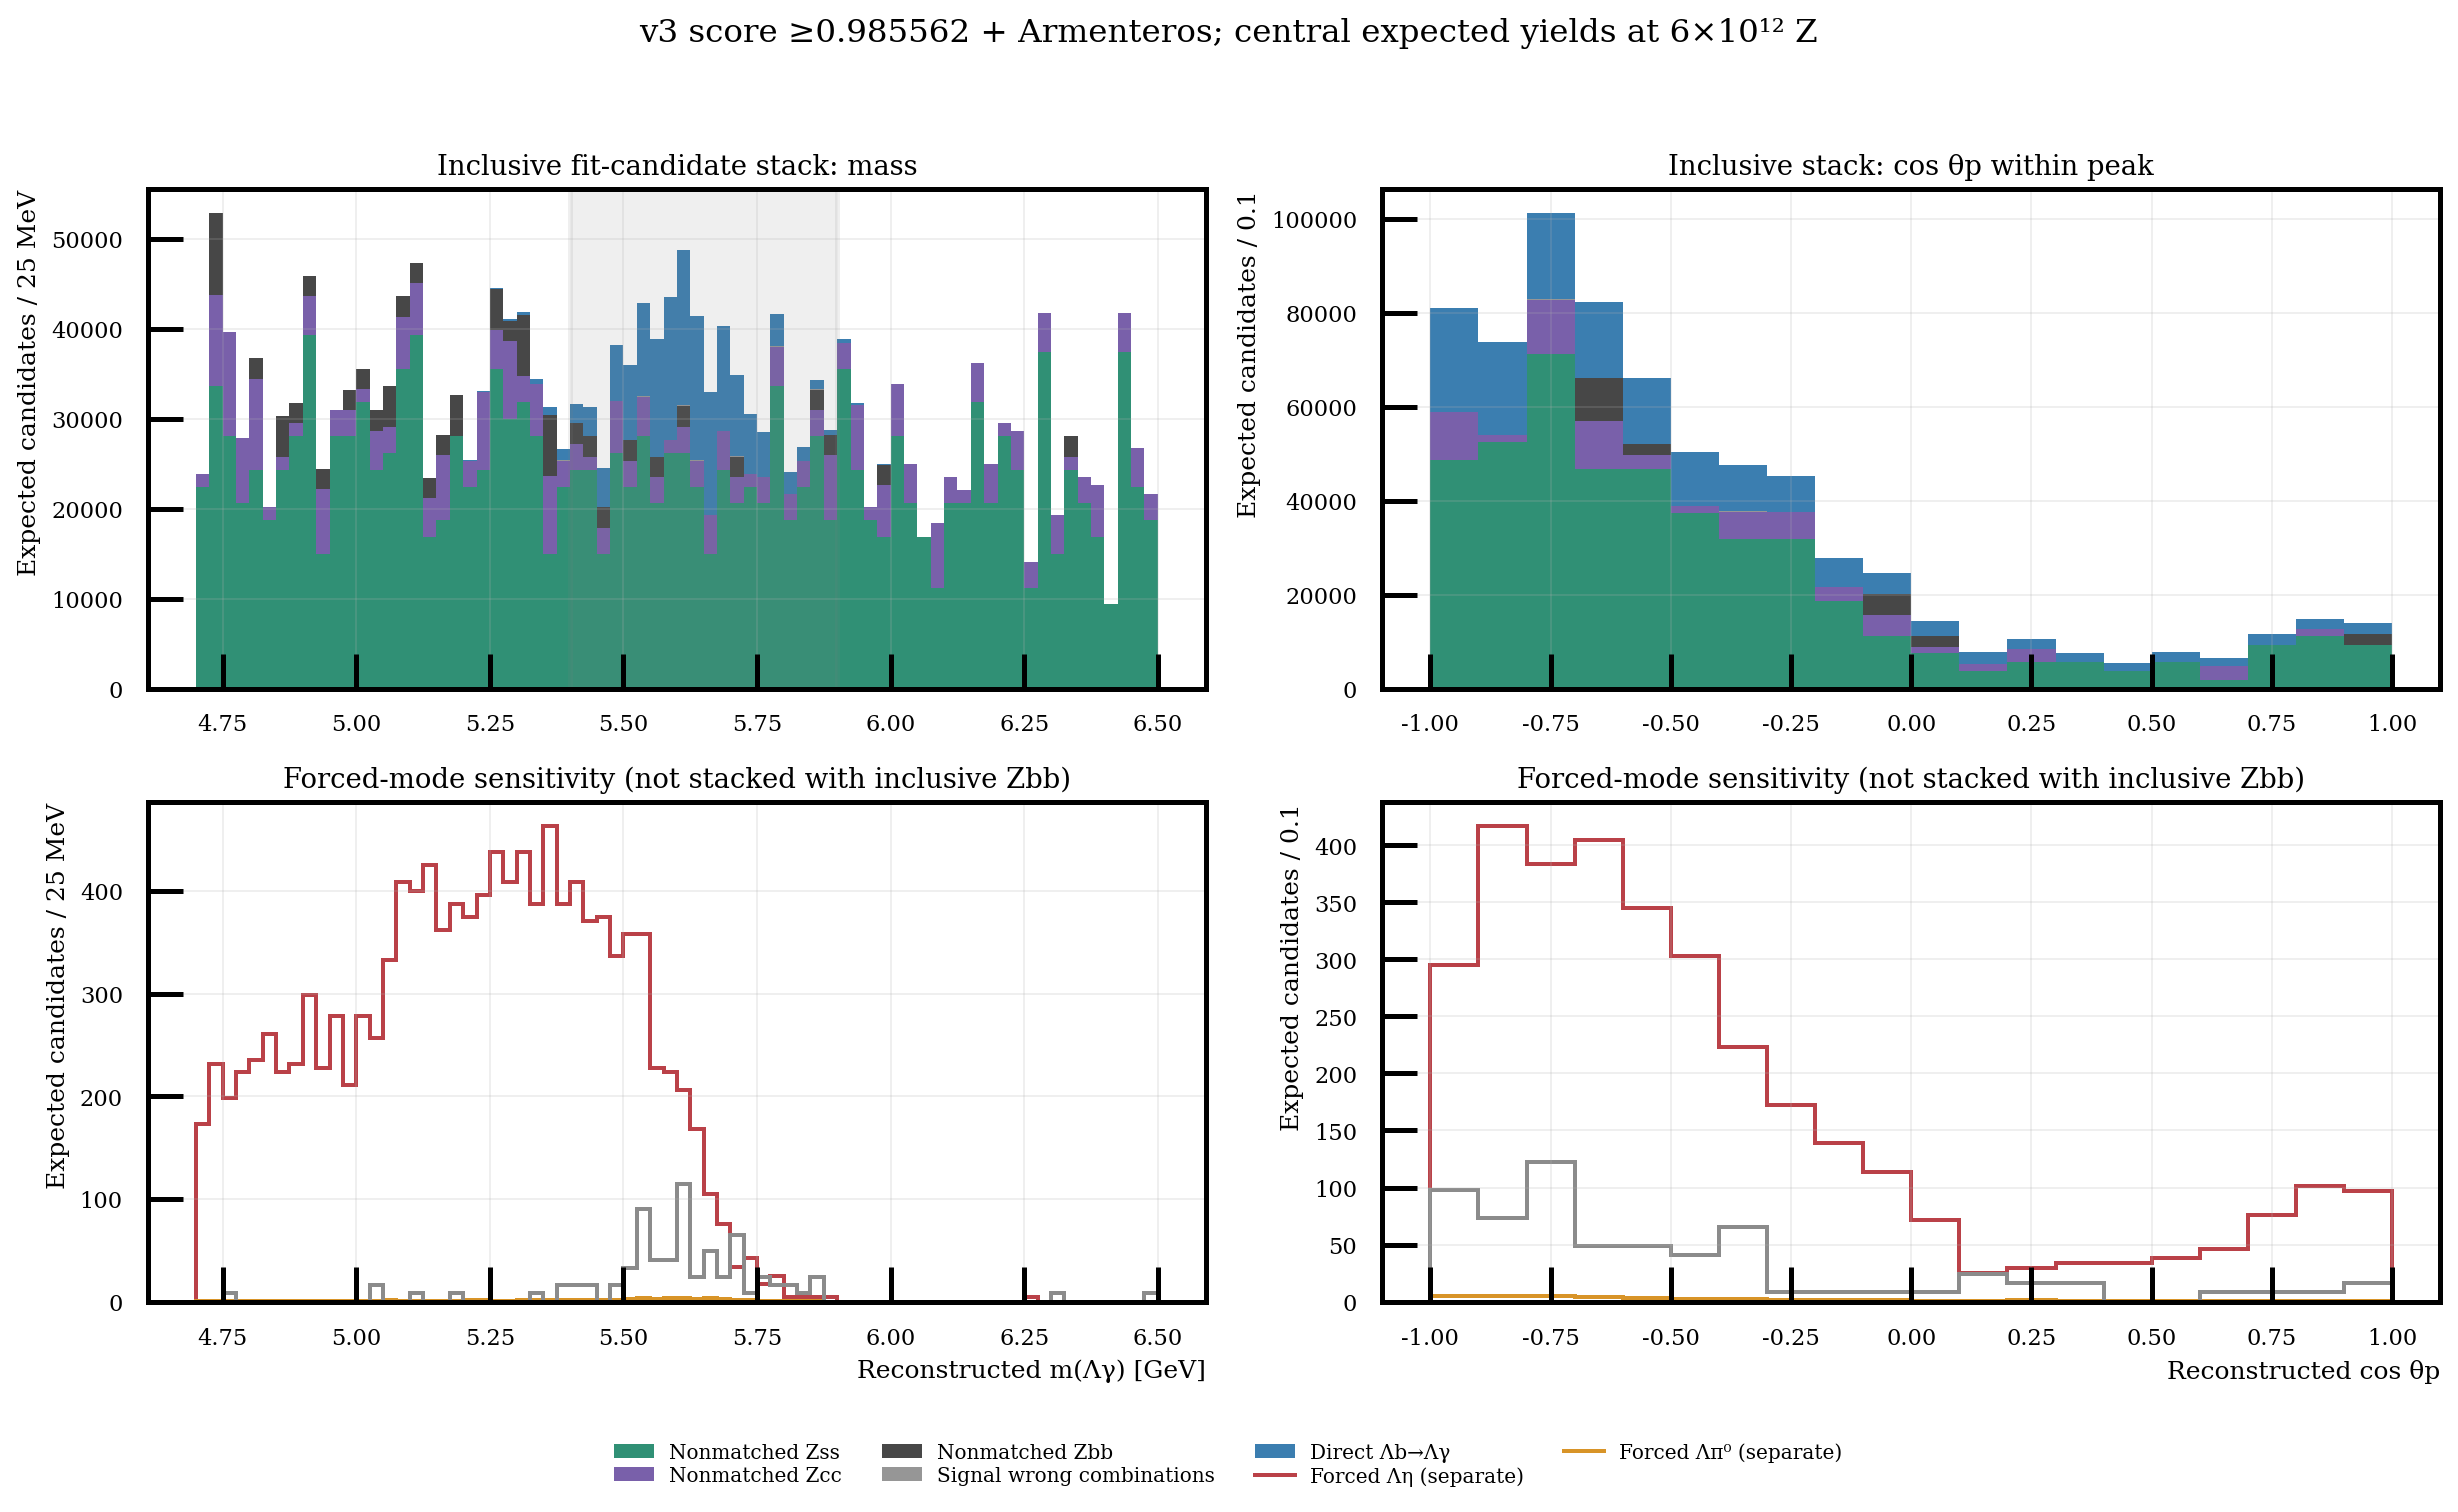
\includegraphics[width=.96\textwidth,height=.75\textheight,keepaspectratio]{figures/reoptimized_arm_only_stack.png}
\scriptsize Linear expected candidate yields: direct signal 152,080; Zbb 20,474; Zcc 66,434; Zss 460,657 in 5.4--5.9 GeV. Wrong combinations 629. Forced $\eta$ 3,347 and $\pi^0$ 39 are plotted separately and excluded from the inclusive stack.
\end{frame}

\begin{frame}{Earlier 0.985562 score: PHSP angular acceptance}
\centering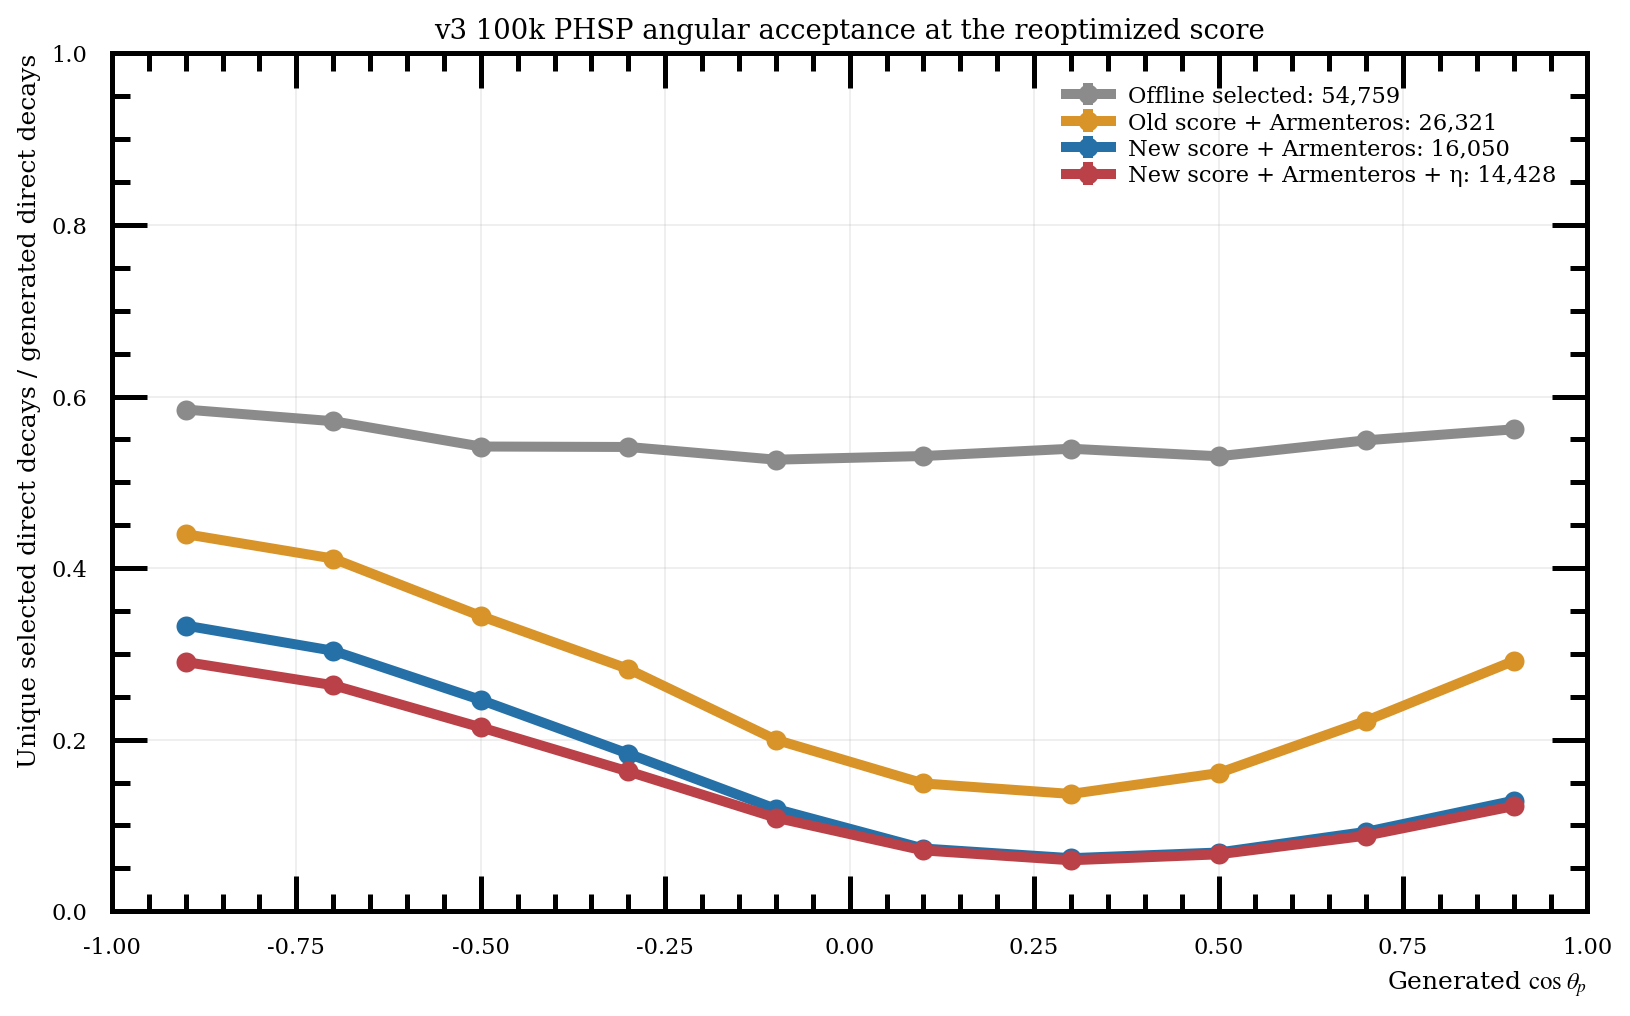
\includegraphics[width=.91\textwidth,height=.68\textheight,keepaspectratio]{figures/phsp_reoptimized_acceptance.png}
\scriptsize Denominator: 100,007 generated direct PHSP decays before any selection. Old score+Armenteros: 26,321 (26.32\%); proposed score+Armenteros: 16,050 (16.05\%). The strong $\ct$ variation requires binned efficiency in an angular fit.
\end{frame}

\begin{frame}{Updated PI objective: high-score $S/\sqrt{B}$}
\begin{itemize}
\item Apply Armenteros to all candidates, then scan the \emph{same Zbb-trained BDT} at high score. Set $B=B_{bb}+B_{cc}+B_{ss}$ with each inclusive flavour physically scaled by its own processed-event count and Z branching scenario.
\item Maximize central $S/\sqrt{B}$ using validation peak rows only. Zero-observed-background points have undefined central $S/\sqrt{B}$; do not call them infinite-significance optima.
\item The Armenteros-only finite validation maximum is \textbf{0.9918887019}; hold that point fixed in the test sample. The precision of the threshold is limited by sparse high-score background MC.
\end{itemize}
\end{frame}

\fig{High-score scan: peak $S/\sqrt{B}$ after Armenteros}{sqrtb_tight_scan.png}

\begin{frame}{Updated high-score expectation in the peak}
\small\begin{tabular}{lrrrrrr}
\toprule
Partition, score & $S$ & Zbb & Zcc & Zss & $B$ & $S/\sqrt B$\\\midrule
Validation, old .953827 & 230,595 & 46,907 & 547,130 & 1,610,856 & 2,204,892 & 155.3\\
Validation, \textbf{.991889} & 108,352 & 23,453 & 14,398 & 206,040 & 243,891 & \textbf{219.4}\\
Test, old .953827 & 229,215 & 78,558 & 404,982 & 1,406,415 & 1,889,954 & 166.7\\
Test at .991889 & 106,504 & 0 & 28,927 & 178,146 & 207,073 & \textbf{234.0}\\
\bottomrule\end{tabular}
\vspace{.7em}

\small Test central $S/\sqrt B$ rises 40.4\% over the old cut. Full-archive descriptive expectation at .991889: $S=108{,}170$, $B=246{,}967$; $S/(S+B)=30.5\%$. Armenteros+$\eta$ test gives 218.8; Armenteros+$\pi^0$ gives 206.3 under this objective.

\scriptsize Validation has only 1 Zbb, 1 Zcc and 11 Zss peak rows at the new point; test has 0, 4 and 19. The test background-upper diagnostic gives $S/\sqrt{B_{\rm upper}}=169.7$ versus 149.9 at the old cut. Branching and detector systematics are not included.
\end{frame}

\begin{frame}{Updated high-score candidate fit view}
\centering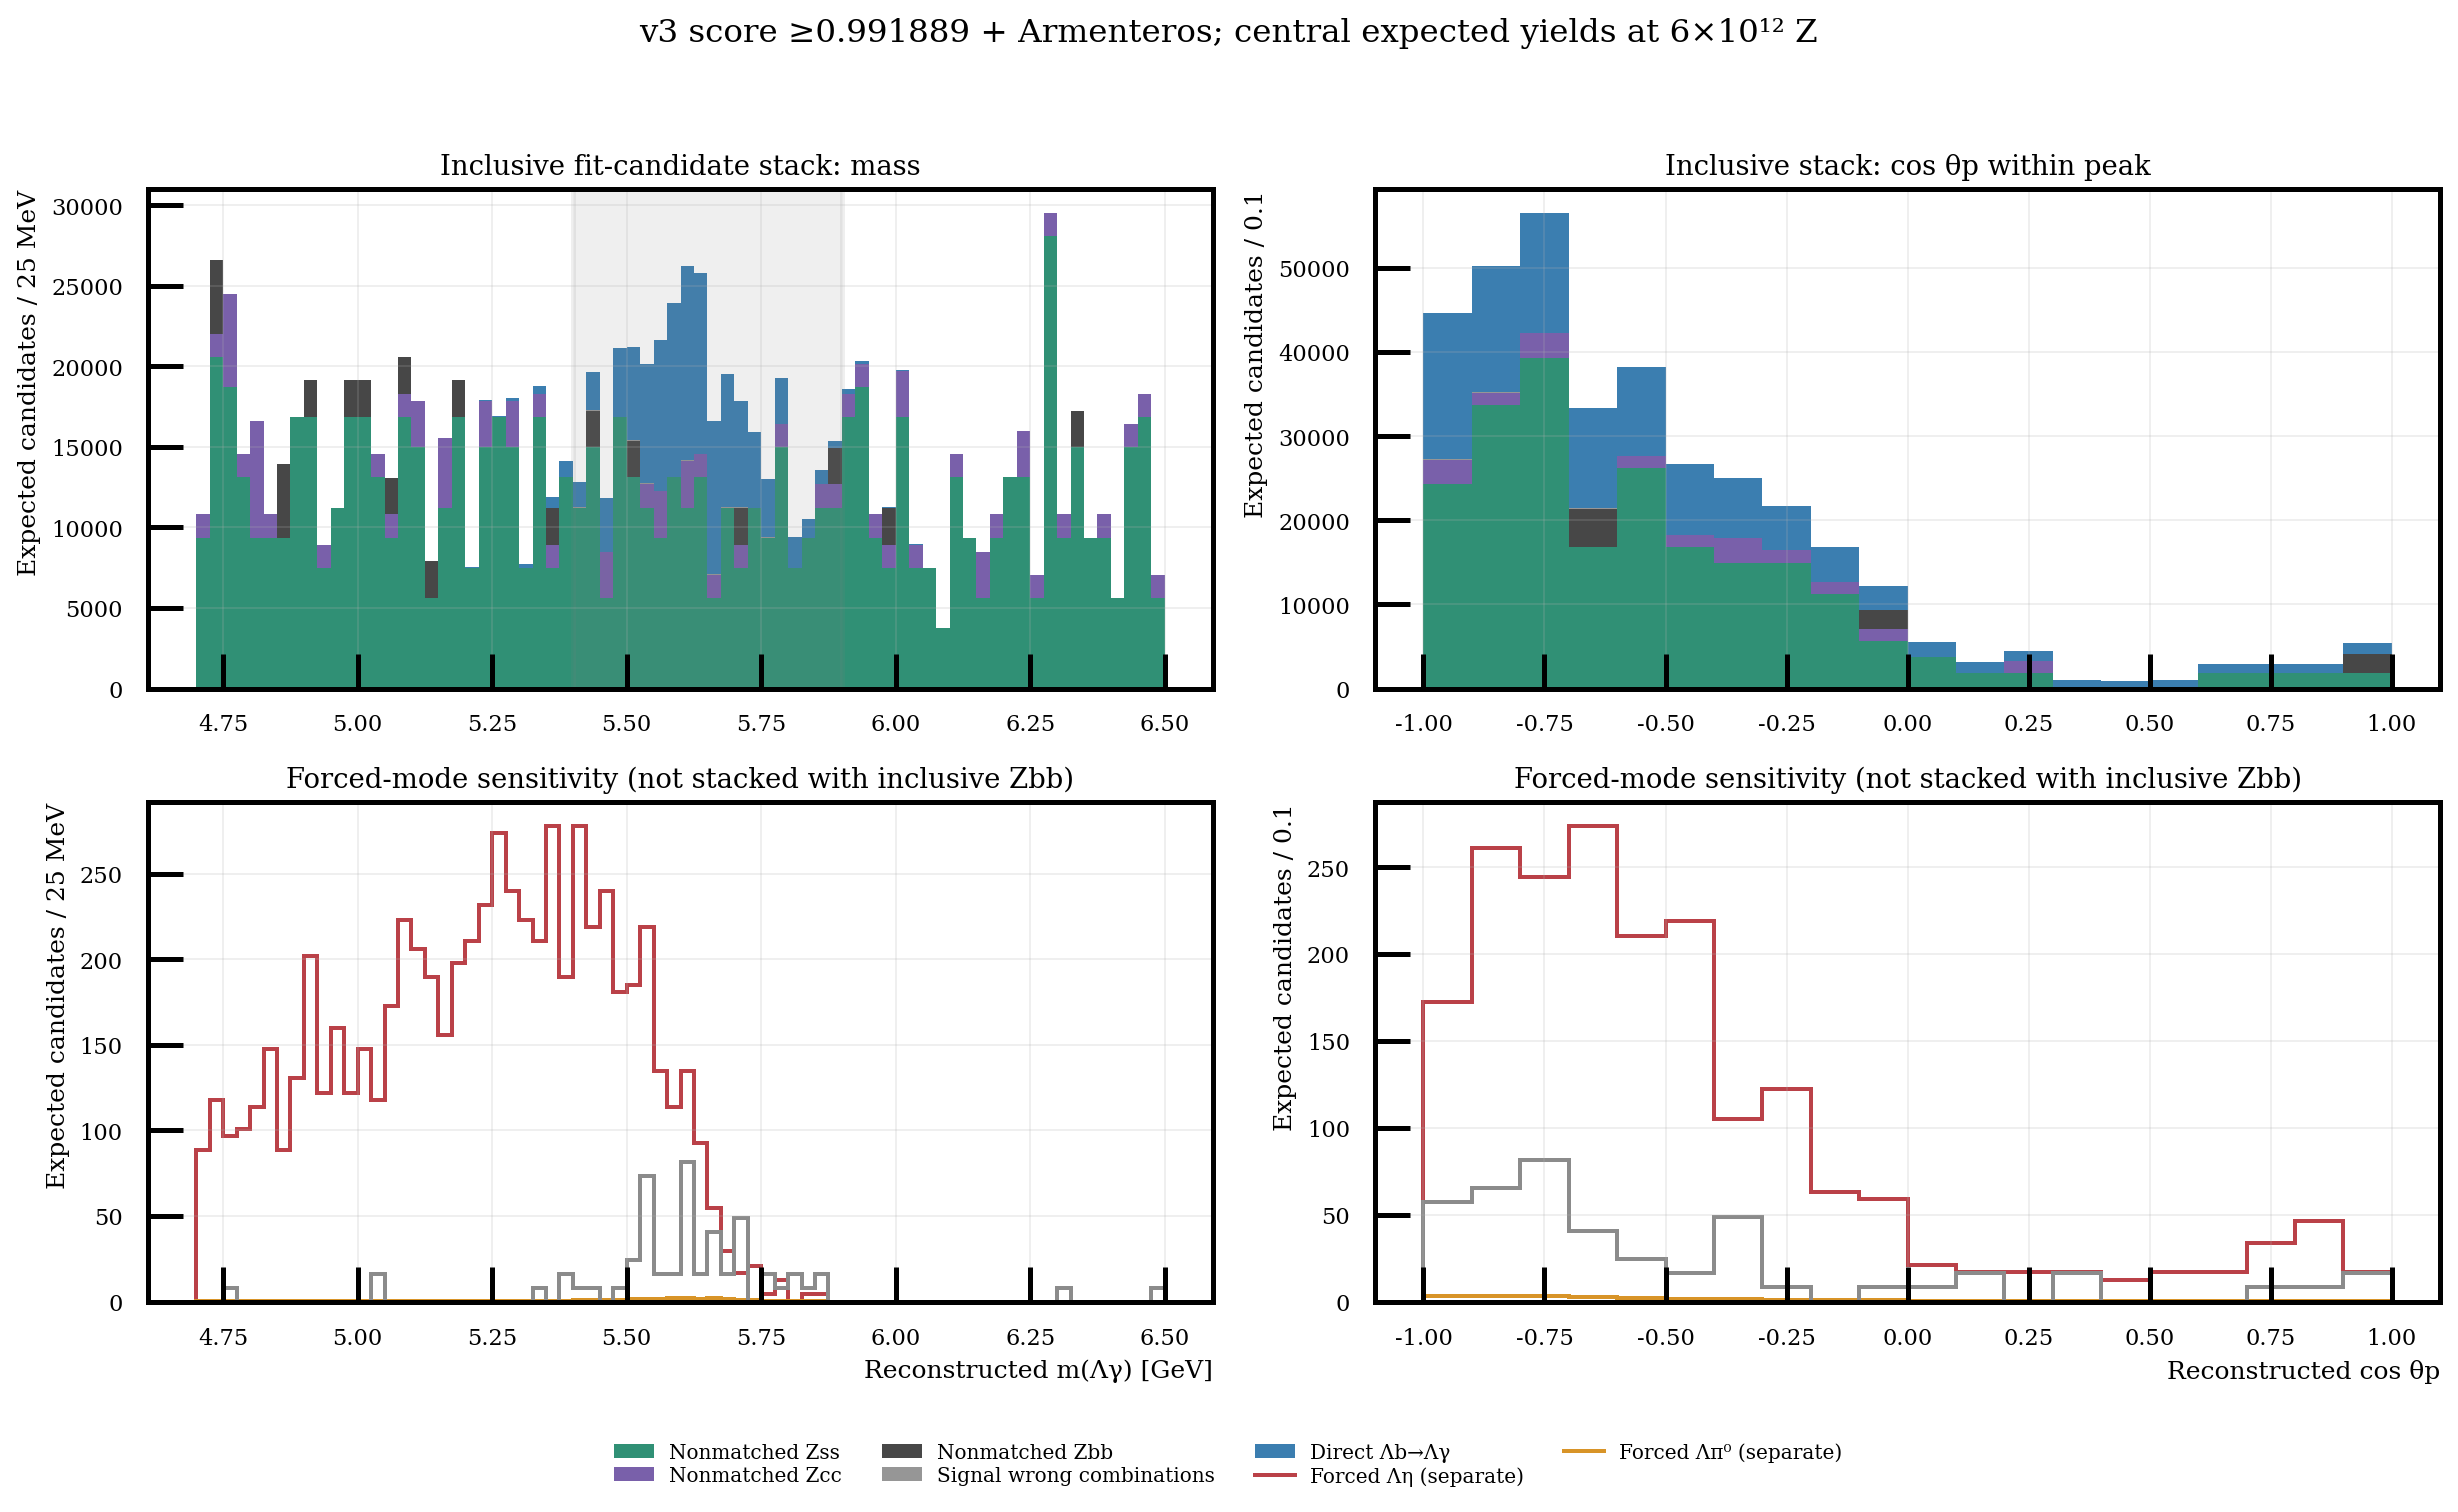
\includegraphics[width=.96\textwidth,height=.75\textheight,keepaspectratio]{figures/sqrtb_stack.png}
\scriptsize Linear expected candidate yields at score .991889 + Armenteros: peak signal 108,170; Zbb 9,100; Zcc 18,775; Zss 219,093. Wrong combinations 425. Forced $\eta$ 1,945 and $\pi^0$ 23 are separate from the inclusive stack.
\end{frame}

\begin{frame}{Updated high-score PHSP acceptance}
\centering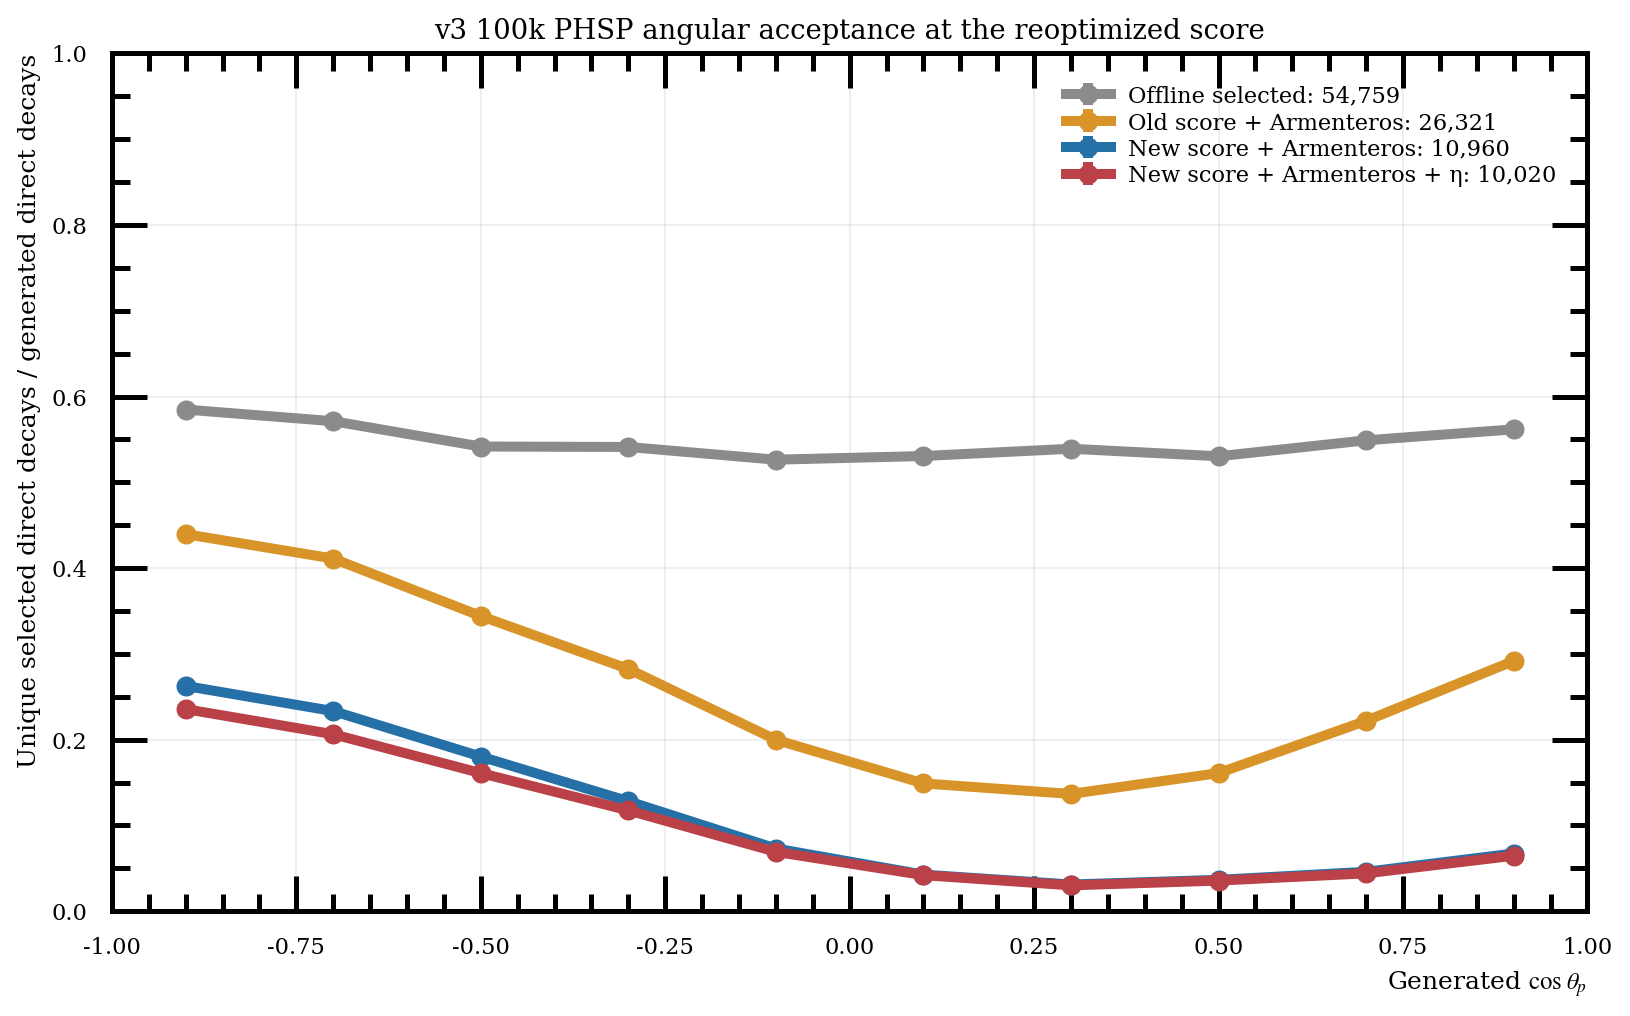
\includegraphics[width=.91\textwidth,height=.68\textheight,keepaspectratio]{figures/sqrtb_phsp_acceptance.png}
\scriptsize Score .991889 + Armenteros selects 10,960 of 100,007 generated direct PHSP decays (10.96\%), versus 16.05\% at .985562 and 26.32\% at .953827. Central 68\% residual half-width is 0.0128; the angular fit requires the binned acceptance and response.
\end{frame}

\begin{frame}{Conclusion and PI decision}
\begin{itemize}
\item The current Zbb-trained BDT can be improved \emph{at the score-selection stage}: the PI-requested peak $S/\sqrt{B_{bb}+B_{cc}+B_{ss}}$ favours score $\geq0.991889$ after Armenteros. Held-out central FoM rises 166.7$\to$234.0; PHSP acceptance falls to 10.96\%.
\item Explicit $\eta$ and $\pi^0$ veto alternatives do not surpass Armenteros alone on the current held-out $S/\sqrt B$ comparison. Armenteros removes most $K_S^0$ fakes, but genuine $\Lambda$ plus photon dominates Zss survivors.
\item The proposed stacked mass/angle distribution is a fit-template starting point. The high-score background tail, branching scenario, possible forced-mode overlap and angular response need further review.
\item Next: compare this score-only result with a weighted Zbb/Zcc/Zss BDT and a named $\Lambda$-displacement feature ablation, using fresh held-out tails and matched signal efficiency. PI to decide the reference selection.
\end{itemize}
\end{frame}

\appendix
\begin{frame}{Backup: exact yield definitions}
\small\[
w_q=\frac{(6\times10^{12})\mathcal B(Z\to q\bar q)}{N_{\rm processed,q}},\quad
S=(6\times10^{12})(0.15)(2)(0.10)(7.1\times10^{-6})(0.639)
\frac{n_{\rm direct}}{N_{\rm generated\ direct}}.
\]
\begin{itemize}
\item The signal numerator counts selected direct candidate rows; PHSP acceptance instead counts unique matched generated direct decays. The two denominators answer different questions.
\item All yield and FoM values shown are in the 5.4--5.9 GeV reconstructed peak; the stack displays 4.7--6.5 GeV mass and peak $\ct$.
\item The quoted FoM has candidate-counting uncertainty but omits systematic terms and correlations. The ss branching fraction is an explicit scenario, not a direct measured input.
\end{itemize}
\end{frame}

\fig{Backup: PHSP reconstructed versus truth $\ct$}{phsp_reoptimized_response.png}

\begin{frame}{Backup: Zss selected-photon ancestor chain}
\centering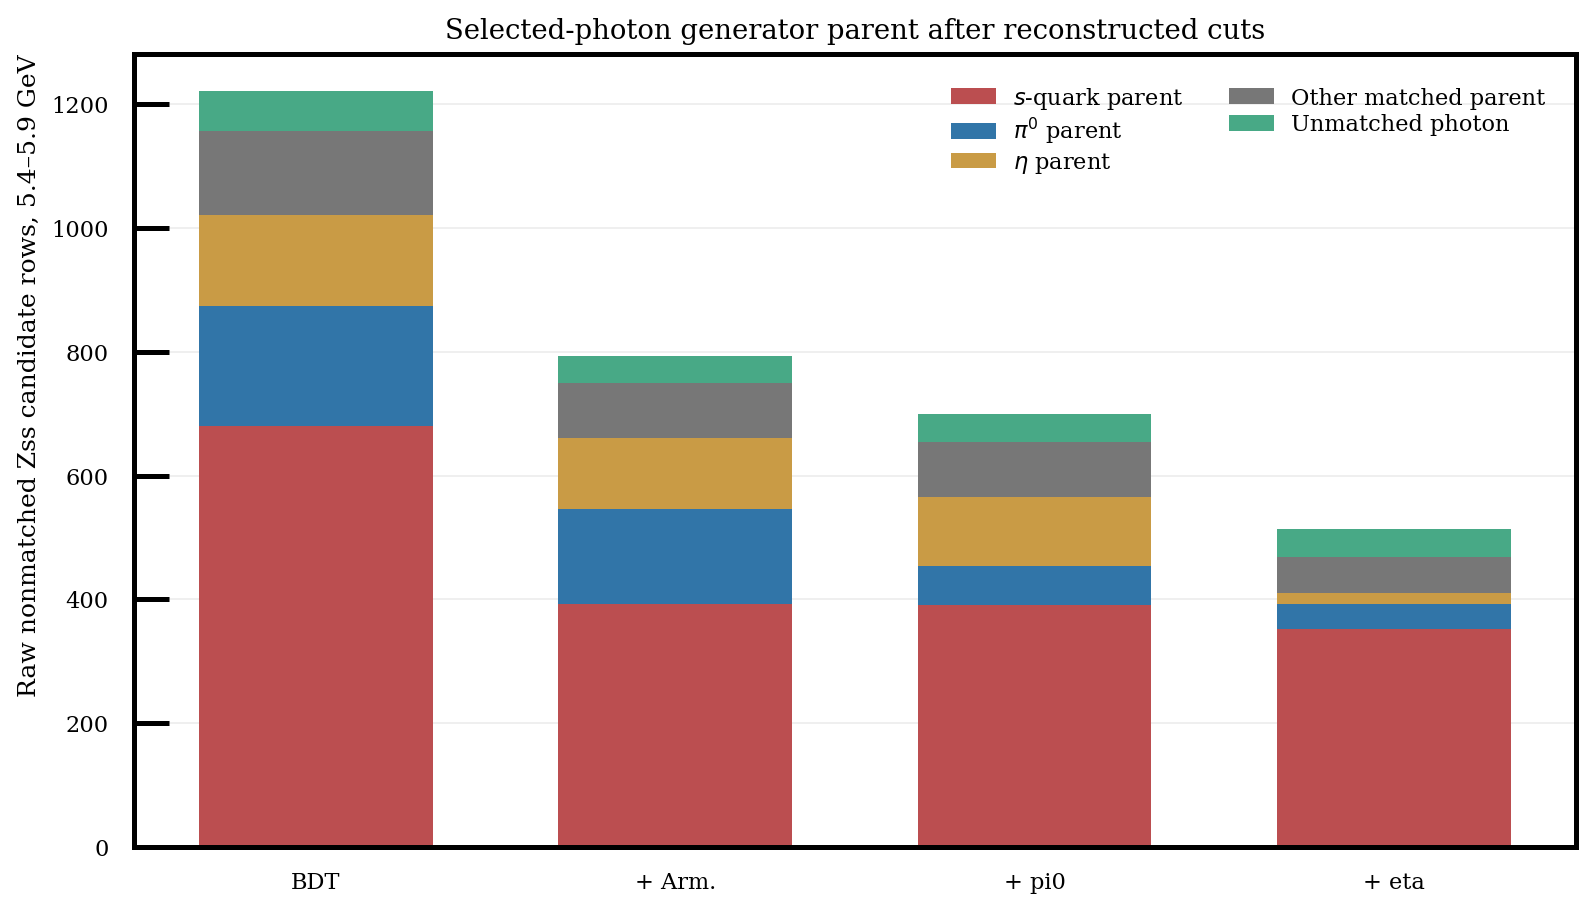
\includegraphics[width=.82\textwidth,height=.68\textheight,keepaspectratio]{figures/zss_peak_photon_source.png}
\scriptsize At old BDT+all vetoes, 352/514 photons have immediate recorded $s$ parent; 347 reach Z in four stored ancestor generations. First-parent ancestry supports a strange-parton origin, but is not a full shower graph.
\end{frame}

\begin{frame}{Backup: Delphes IDEA charged-track acceptance}
\small\begin{tabular}{lrrr}
\toprule
Truth-bin population & Generated & Unique reco match & Fraction\\\midrule
Charged $p_T\geq0.1$ GeV, $|\eta|<2$ & 207,781 & 203,634 & 98.0\%\\
$2\leq|\eta|<2.56$ & 5,838 & 5,382 & 92.2\%\\
$|\eta|\geq2.56$ & 2,028 & 0 & 0\\
Fiducial $\Lambda\to p$ & 594,874 & 508,767 & 85.5\%\\
Fiducial $\Lambda\to\pi$ & 577,517 & 486,799 & 84.3\%\\
Fiducial $K_S^0\to\pi$ & 575,230 & 566,990 & 98.6\%\\
\bottomrule\end{tabular}
\vspace{.7em}

\scriptsize Historical 500k Gamma Delphes response audit; truth-bin matching with unique MCRecoAssociation, not a v3 Stage 1 cutflow. Source: \texttt{studies/resolutions/FINDINGS.md}. The measured match fraction includes geometry, reconstruction and association effects.
\end{frame}

\begin{frame}{Backup: displacement and track-resolution checks}
\small\begin{itemize}
\item In the same 500k Delphes audit, $\Lambda$ protons have unique-match fraction 98.7\% for production $R_{xy}=209$--520 mm, 93.2\% for 520--1,296 mm, 45.2\% for 1,296--3,226 mm and 0 beyond 3,226 mm. Displaced acceptance needs explicit validation for topology cuts.
\item Charged tracking card input: $p_T\geq0.1$ GeV, $|\eta|\leq2.56$, 2 T field, layered TrackCovariance geometry/material, at least six hits. No single scalar momentum-resolution formula is assumed.
\item Resolution audit fits Gaussian cores of $(p_{\rm reco}-p_{\rm true})/p_{\rm true}$ and $p_T$ analogues versus truth $p_T$, signed $\eta$ and production radius, using only unique matches. The archived numerical resolution plots are unavailable in this checkout; no widths are inferred from card inputs here.
\end{itemize}
\scriptsize Source and reproduction scripts: \texttt{studies/resolutions/FINDINGS.md}, \texttt{run\_study.py}, \texttt{run\_displaced\_daughters.py}, \texttt{run\_comparison.py}.
\end{frame}
\end{document}
